
\documentclass[12pt]{article}
\usepackage{graphicx} % for including images
\usepackage{hyperref} % for creating hyperlinks
\usepackage{amsmath} % for mathematical expressions
\usepackage{lipsum} % for generating dummy text
\usepackage{listings} % for code blocks
\usepackage{float} % place images where they appear in the LaTeX

\lstset{
  language=bash,
  basicstyle=\ttfamily,
  breaklines=true
}

\begin{document}
% Title page information
\title{Raspberry Pi 4 Environment Configuration}
\author{Jaidon Lybbert, University of Washington}
\date{January 24, 2024}

% Generate the title page
\maketitle

% Abstract section
\begin{abstract}
This report documents the setup and configuration of a portable development environment for a headless Raspberry Pi 4 on a cellular hotspot. The environment consists of a Windows 10 laptop, iPhone 13 Pro, and Raspberry Pi 4B. The Pi is pre-configured with the SSID and password to connect to the iPhone hotspot, and accessed from the laptop through SSH. The Pi is set up with the Neovim editor for on-device development, with language support for Python, Rust, C, C++, and Zig. For debugger support, the Windows laptop is set up with Visual Studio and VSCode with extensions for the same languages.
\end{abstract}

% Introduction section
\section{Introduction}
This document is organized as follows. In Section \ref{sec:background} I describe my experience with embedded systems and software, motivations and intent, and take a look at the physical interface to the Raspberry Pi 4. I devise a plan for setting up my preffered environment in Section \ref{sec:methods}, describe what the actual environment ends up looking like in Section \ref{sec:results}, and discuss the failures and hurdles I faced in Section \ref{sec:discussion}. I conclude in \ref{sec:conclusion} by discussing the improvements I would like to make in the future.

% Methods section
\section{Background}\label{sec:background}
\subsection{Programming Experience}
I graduated with my BS in Electrical Engineering at Eastern Washington University in 2022, with a concentration in Embedded Systems. As part of my coursework, I programmed an FPGA in VHDL to implement a processor supporting a subset of the MIPS instruction set. I did several small projects using the TI ARM\textregistered{} Cortex\textregistered-M4F Based TM4C123G LaunchPad\texttrademark{} MCU evaluation board \cite{ti_ek_tm4c123gxl}, and was introduced to real-time operating systems using the Arduino Mega which I used to make a kitchen timer\cite{lybbert2023} with polling and pre-emptive scheduling.

While at EWU, I was an officer in the IEEE Student Chapter, and made a controller for a skittle-sorting machine, again using the TM4C123G \cite{sorter_project}. 

For two years, I worked at an aerospace startup developing real-time control software for a pressurized gas system using an Allen-Bradley PLC. 

I spent the summer of 2022 doing an internship at SpaceX, where I developed tools in Python to automate workflows and manage parts data.

My graduate studies have been in high-performance parallel computing on the NVIDIA Cuda platform, with some graphics programming in OpenGL and Vulkan, and some deep neural networks. My most recent work has been developing a parallel QR decomposition algorithm with Amazon Lab126 for in-home robotics applications\cite{mixed_precision}.
\subsection{Experience with the Raspberry Pi}
I have done some projects with the Raspberry Pi 3B, and Raspberry Pi-ZeroW. For a time, I had the Raspberry Pi 3B set up as an ad-blocking DNS server using the Pi-hole project \cite{pihole}, and I used the ZeroW for a weather station project as an undergrad in IEEE \cite{weatherstation}.
\subsection{Motivation}
My experience with bare-metal programming and parallel programming on GPUs has given me a great appreciation for on-device debuggers, and memory management. My recent interests have been in programming languages themselves, and the tradeoffs they offer. At the same time, I have been becoming more mobile, and work in a variety of places from my laptop, leaving the desktop, two monitors, and mouse at home. The single low-res screen and trackpad have led me down the path of keyboard shortcuts, macros, and Neovim to ergonomically switch between windows and edit code without using the trackpad. 

These motivations form the basis of the requirements for my development environment (plus version control as a given). 

\begin{itemize}
  \item Portability
  \item Version control
  \item Support for several languages
  \item On-device debugging
  \item Compatibility with Neovim
\end{itemize}


\section{Methods}\label{sec:methods}

\subsection{Installation}
The Raspberry Pi 4B is a relatively simple device to setup following the documentation \cite{raspberrypi_config}. I used a 16GB SD card and flashed the 64-Bit Raspberry Pi OS "Bookworm" to it on my Windows 10 laptop with the provided Raspberry Pi Imager tool. I took a screenshot of the hostname and username configuration, so I wouldn't forget it.

\subsection{Portability}
In advanced settings in the Imager tool, the pre-configured WiFi network was automatically filled, along with the public SSH key from my laptop. I changed the SSID and password for the WiFi network to my iPhone hotspot so I have the option to physically bring my Pi with me and connect with SSH. 

\begin{figure}[H]
\centering
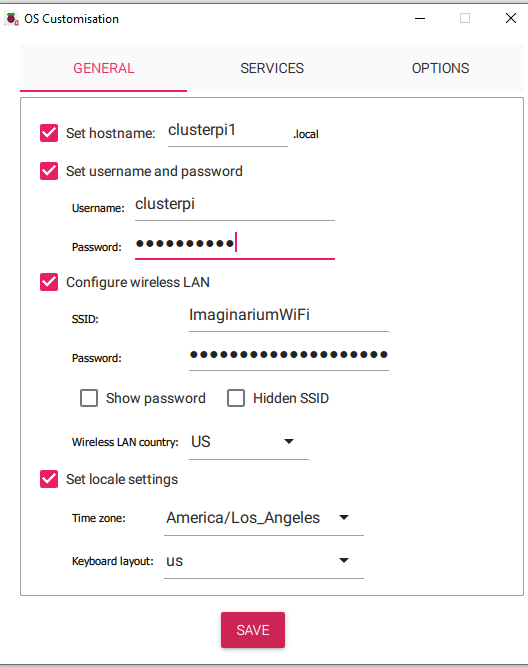
\includegraphics[width=0.75\textwidth]{raspiconfig.png} % replace with your own image file
\caption{The Raspberry Pi Imager showing hostname and username configuration.}
\label{fig:raspiconfig}
\end{figure}

The Pi connected to the hotspot on boot without issue, and I was able to SSH into it by the hostname. I immediately scanned for my home WiFi network, and added it with higher priority using the Network Manager CLI. Switching networks caused the SSH session to hang, but switching networks on my laptop and restarting the SSH connection went without issue.

\begin{figure}[h]
\centering
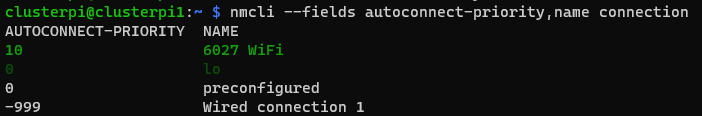
\includegraphics[width=1.0\textwidth]{network-config.png} % replace with your own image file
\caption{WiFi network prioritization in Network Manager. The mobile hotspot was labeled "preconfigured" by default, the home network is named by the SSID "6027 WiFi".}
\label{fig:networkpriority}
\end{figure}

I updated the Pi with APT through my home network. 

\subsection{Version Control}

Once my packages were up to date, I generated an SSH key pair with \verb|ssh-keygen| and copied the public key to my personal Github account. I created a new repository \cite{lybbert2024classwork} and cloned it to the Raspberry Pi. 

cd ~
git clone git@github.com:jaidonlybbert/EEP522A-W24.git

\subsection{Language Support}

At this point I checked the remaining space on my SD card with the \verb|df -H| command. I would keep an eye on it as I began installing packages.

\begin{figure}[h]
\centering
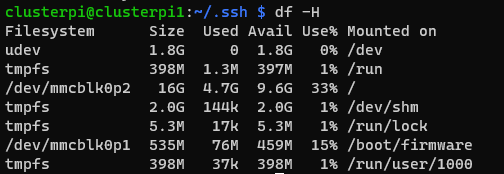
\includegraphics[width=1.0\textwidth]{freespace.png} % replace with your own image file
\caption{Free space on the SD card after basic installation. The filesystem has ~9GB available.}
\label{fig:freespace}
\end{figure}

The full set of languages I want to support are:
\begin{itemize}
  \item Python
  \item Rust
  \item C
  \item Zig
  \item C++
\end{itemize}

I found GCC and Python came pre-installed with the OS. 
I installed Rust by fetching and executing the installer with the one-liner 
\begin{lstlisting}
curl --proto '=https' --tlsv1.2 -sSf https://sh.rustup.rs | sh
\end{lstlisting}
as suggested by the docs \cite{rust_installation}.

I attempted to compile Zig from source using the zig-bootstrap \cite{zig-bootstrap} repository. The only dependency missing to compile Zig was CMAKE, which I planned to install anyway. I installed Ninja as well to speed up the build process.

I got the triplet for the raspberry pi using

\begin{lstlisting}
gcc -dumpmachine
\end{lstlisting}

I set the CMAKE environment variable to use Ninja instead of Make.

\begin{lstlisting}
export CMAKE_GENERATOR=Ninja
\end{lstlisting}

Then ran the build script for Zig

\begin{lstlisting}
./build aarch64-linux-gnu native
\end{lstlisting}

It occured to me as the build spooled up that this was the first real workload I put on the device. I gave the small adhesive heatsink I put on the SoC an ill-advised finger test and determined it was getting hot. As it turns out the Pi is quite slow relative to the size of the job of compiling Zig. It would take several hours. After looking at the repository again, I realized that I wasn't just compiling Zig, I was also compiling LLVM, LLD, Clang, zlib, and zstd. Ultimately, the build failed when my laptop went into hibernate mode and the SSH session disconnected.

I went the easy route and just downloaded the released binary for the aarch64 architecture. 

\begin{lstlisting}
wget https://ziglang.org/builds/zig-linux-aarch64-0.12.0-dev.2338+9d5a133f1.tar.xz 
\end{lstlisting}

\subsubsection{Neovim Setup on Device}
A development environment is set up on the device using Neovim with language support for Python, Rust, C, C++, and Zig. By default, Neovim supports syntax highlighting for these languages, for code completion and static analysis, language-specific plugins are added. 

\subsubsection{VSCode} A VSCode-based development environment is set up on the Windows 10 machine for instances when a debugger is necessary, with extensions for Python, Rust, and Zig. These extensions add syntax highlighting, language servers, and linting to VSCode.
\begin{itemize}
\item Python - Microsoft
\item rust-analyzer - The Rust Programming Language
\item Zig Language - ziglang
\item Zig Language Extras - Igor Anic
\end{itemize}

\subsubsection{Visual Studio}
Visual Studio is used for C and C++, since those projects are built with MSBuild through CMAKE, which outputs Visual Studio projects. I installed the Visual Studio 2022 Community Edition.

\subsubsection{Hello World!}
I created a "src" directory in my repository, and a subdirectory for a "hello world" app in each language.

\begin{lstlisting}
mkdir ~/EEP522A-W24/src 
cd ~/EEP522A-W24/src
mkdir hello_python hello_c hello_rust hello_zig
\end{lstlisting}

From inside each folder I initialized a "hello world" project with their respective methods.

\paragraph{Python}
For Python I simply created a .py file with Neovim and put a single "hello world" print statement in it, then ran the file with the interpreter.

\begin{lstlisting}
nvim hello_world.py
python hello_world.py
\end{lstlisting}

\paragraph{Rust}
Rust uses Cargo to build and run applications. Initializing a new Cargo package creates a "hello world" application by default.

\begin{lstlisting}
cargo new hello_rust
cd hello_rust
cargo run
\end{lstlisting}

\paragraph{C}
For C, I asked Bing Chat to "create a template CMakeLists.txt for a single c file called 'hello.c'" and pasted the response with Neovim.
I asked Bing Chat to "create a hello.c program in C which prints 'hello world!'" and pasted the response.

\begin{lstlisting}
nvim CMakeLists.txt
nvim hello.c
\end{lstlisting}

Then ran CMake to build the project on the device.

\begin{lstlisting}
mkdir build
cd build
cmake ..
cmake --build .
\end{lstlisting}

The project compiled with GCC and ran without issue.

\begin{lstlisting}
./Debug/HelloWorld
\end{lstlisting}

I repeated the CMake build process on my Windows machine, and verified the build worked correctly with MSBuild.

\paragraph{Zig}

\subsubsection{Debugger Test}
I opened the ./src/ folder of my repository in VSCode on my Windows machine and set a breakpoint at the first line of each "hello world" program for Python, Rust, and Zig. I verified that the debugger was working for each one. For C, I opened the built project in Visual Studio, set a breakpoint and ran the project in Debug mode to verify the debugger was working.

\subsubsection{Profiling Challenge}

I created a new directory in my repository called "data".

\begin{lstlisting}
mkdir ~/EEP522A-W24/data
cd ~/EEP522A-W24/data
\end{lstlisting}

I downloaded the \verb|.zip| file from our class Canvas page to the repository on my Windows machine and pushed it to Github, then pulled the changes on the Pi.

I extracted the folder.

\begin{lstlisting}
extract ee_course.zip
\end{lstlisting}

I ran the shell script without changes to see the output.

\begin{lstlisting}
./ee_course/run.sh
\end{lstlisting}

Following the guide in the assignment instructions I opened the \verb|prototype.c| file in Neovim and jumped to the \textit{void prototype translate information(char * model)}  function. From the output of the program in it's broken state, I deduced that I needed to copy the board details, which are output by the command

\begin{lstlisting}
cat /proc/cpuinfo
\end{lstlisting}

To the \verb|g_core| struct.

\begin{figure}[h]
\centering
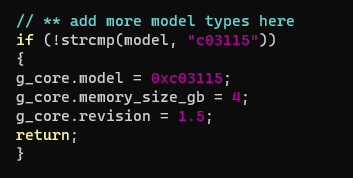
\includegraphics[width=0.5\textwidth]{prototype_edit.png} % replace with your own image file
\caption{Code added to 'prototype.c' for raspberry pi 4 support.}
\label{fig:prototype_edit}
\end{figure}

I re-ran the shell script, pushed results to GitHub, and pulled them down to my laptop to look at.

% Results section
\section{Results}\label{sec:results}

The images produced by the experiment are shown in Figures \ref{fig:plot_memlib}, \ref{fig:plot_memsys}, and \ref{fig:plot_time}.

\begin{figure}[htbp]
\centering
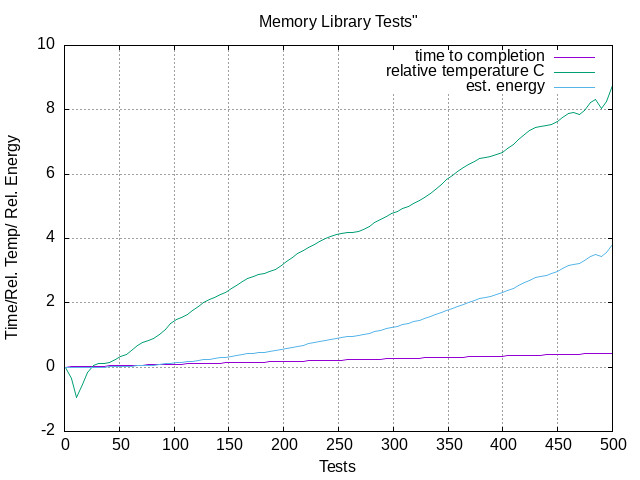
\includegraphics[width=1.0\textwidth]{../../data/ee_course/plot_memlib.jpg} % replace with your own image file
\caption{Output of the Memory Library test.}
\label{fig:plot_memlib}
\end{figure}

\begin{figure}[htbp]
\centering
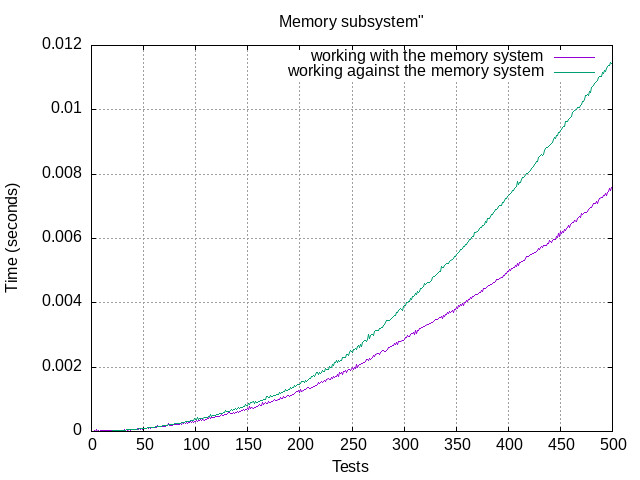
\includegraphics[width=1.0\textwidth]{../../data/ee_course/plot_memsys.jpg} % replace with your own image file
\caption{Output of the Memory Subsystem test.}
\label{fig:plot_memsys}
\end{figure}

\begin{figure}[htbp]
\centering
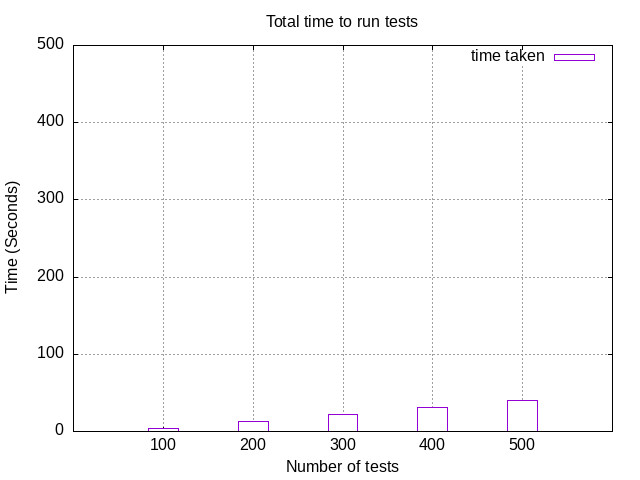
\includegraphics[width=1.0\textwidth]{../../data/ee_course/plot_tests.jpg} % replace with your own image file
\caption{Output of the execution time test.}
\label{fig:plot_time}
\end{figure}

% Discussion section
\section{Discussion}\label{sec:discussion}

\subsection{Interpretation of Graphs}
Figure \ref{fig:plot_memlib} shows the correlation of time, temperature, and energy use relative to the number of memory tests performed. Although the units are not clear, what is clear is that temperature increases almost linearly with number of tests, while energy use is nearly exponential.

Figure \ref{fig:plot_memsys} shows the difference in execution time that optimizing memory access patterns can make. By "working with the memory system" total execution time can be dramatically reduced. 

Figure \ref{fig:plot_tests} shows execution time compared the number of tests performed. In this one, changing the y-axis scaling would improve readability. The obvious takeaway is that more tests take more time. 

\subsection{Issues Encountered}
\subsubsection{Initializing WiFi}
I initially tried installing the Raspberry Pi OS using the same method I had used for the Raspberry Pi 3B several years ago. It used to be the case that you could pre-configure the WiFi connection by flashing the image to the SD card, then copying a \verb|wpa_supplicant.conf| file to the boot partition before installing it to the device. This is no longer supported by the "Bookworm" Raspbery Pi OS and onwards \cite{raspberrypi_config}. 

\subsubsection{Compiling Zig from Source}
Compiling Zig turned out to be more computationally intensive than I expected, and my SSH session was terminated by my host machine going into hibernation mode. If I were to try it again, I would install a fan on the Pi, and use a session manager like \verb|tmux| to preserve the compilation process after disconnecting my SSH session.

% Conclusion section
\section{Conclusion}\label{sec:conclusion}
The result of this work is a headless Raspberry Pi set up with prioritized WiFi connections to a mobile hotspot, and my home network. I am able to edit code with syntax highlighting, code completion, and "peak definition"-type functions using a modified configuration of Neovim on the device through an SSH connection. My code is synced to GitHub, and I am able to transfer and step-debug code on my Windows machine. Python, Rust, Zig, C, and C++ are supported by the environment.

I fell short of being able to do on-device debugging. This could become a problem if I start programming using significant device-specific code. In the future, I would like to explore using GDB directly through the shell for some basic debug functionality, and explore other options for dumping memory regions for analysis.

% Bibliography from refs.bib
\bibliographystyle{plain}
\bibliography{refs}

\end{document}
